 \documentclass[12pt,letterpaper]{article}
 
 % Insert package usage statements here:
 \usepackage{listings}
 \usepackage{graphicx}
 
 \begin{document}
 
 \title{The Nudge Support Toolset}
 \author{Michael A. Gohde}
 \date{December 6, 2016}
 \maketitle
 
 \section{Overview}
 The task of writing stories for Nudge is inherently difficult. The Nudge
 Support Toolset exists to alleviate some of this difficulty by providing
 a large set of utilities designed to compile, validate, and install stories.
 
 This document exists to detail the function and operation of each utility
 in the Nudge Support Toolset.
 
 \section{story2xml.py}
 story2xml exists to translate well structured, human-readable stories into 
 an intermediate XML format for use by all of the other tools in the set.
 
 \subsection{Input file format}
 \lstset{numbers=left, frame=shadowbox}
 \begin{lstlisting}
 Title: <Insert story title here>
 
 First story node title:
    <Insert story node text here>
    
    Responses:
        Response 1 text -> prb1% to dst1, prbN% to dstN
        Response N text -> prb3% to dst3
 \end{lstlisting}
 
 Each story2xml input file must follow a common set of conventions:
 \begin{enumerate}
   \item The story's title must be written on its own line and prefixed with ``Title:''
   \item Each story ``block'' or ``decision'' (hereafter referred to as a ``node'') must start with a title followed by a colon.
   \item The text content in each node (ie. the story text) must not start with a word followed by a colon.
   \item All possible user actions are defined in a block prefixed by the keyword ``Responses:''. This block must be indented more than all of the other text in its node.
   \item Every story must be terminated with a reference to a node named ``END''. This node should not be defined, but exists as a special destination.
 \end{enumerate}
 
 \subsection{A complete input file example}
 \begin{lstlisting}
Title: Example story

D1_0:
    You are confronted with a serious question: 
    To cheese it or not to cheese it?
    
    Responses:
        Cheese it! -> 50% to D2_0, 50% to D2_1
        Don't cheese it! -> 100% to D2_2

D2_0:
    Note: This is a comment.
    Note: All comment text is discarded.
    
    You were able to cheese it!
    
    Responses:
        Proceed -> 100% to D3_0

D2_1:
    Comment: This is also a comment.
    You were unsuccessful at cheesing it!
    
    Responses:
        Proceed -> 100% to D3_0

D2_2:
    You proceed not to cheese it.
    
    Responses:
        Proceed -> 100% to D3_0
        
D3_0:
    Regardless of whether you cheesed it, 
    something happened.
    
    Responses:
        End -> 100% to END
 \end{lstlisting}
 
 \subsection{Running story2xml}
 story2xml accepts one argument on the command line: the name of a text file containing a properly formatted story.
 Once run, story2xml will print an XML-formatted story to stdout, so it may be useful to redirect its output to a different
 file. 
 
 Example usage:
 \begin{center}
 story2xml.py mystory.txt $>$mystory.xml
 \end{center}
 
 \subsection{Error messages}
 When compiling a story, story2xml attempts to perform a few tests to ensure that the provided source file is logically sound.
 If an error is encountered, story2xml will print a message and information that can be used to locate and correct the error.
 
 List of error messages:
 \paragraph{Error: for response (response text) on line (line number), destination probabilities exceed 100\%}
 This error indicates that the total of all of the weights for some response exceeds 100\%. To correct this error, go to the line indicated and re-evaluate all weights.
 \paragraph{Error: for response (response text) on line (line number), destination probabilities sum to a value below 100\%}
 This error indicates that the total of all o fthe weights for some response is below 100\%. To correct this error, go to the line indicated and re-evaluate all weights.
 \paragraph{Warning: for line (line number), unknown token (string)}
 This message indiciates that the compiler has found a command (a word followed by a colon) that it has no rule to handle. This can safely be ignored in some cases.
 
 \section{sanitytext.py}
 sanitytest exists to check whether a story is logically complete by a number of metrics. These include whether a story can be finished through every possible
 combination of user actions, whether every set of weights sums to 100\%, and whether there are any circular references within a story. 
 
 \subsection{Running sanitytest}
 Like story2xml, sanitytest accepts one argument on the command line: the nane of a text file containing an XML-formatted story file.
 When run, sanitytest will either produce an error output or a message indicating that the story passed all checks.
 
 Example usage:
 \begin{center}
 sanitytest.py mystory.xml
 \end{center}
 
 \subsection{Example output}
 \begin{lstlisting}[breaklines=true]
user@computer-$ ./sanitytest.py ../examples/err.story.xml
Circular reference check failed for node D1_0 referred to by D2_1
 \end{lstlisting}
 
 \subsection{Error messages}
 When performing checks on a story, sanitytest my produce one of several error messages. Each error message 
 specific directions as to the nature of the error and where it is in the story.
 
 \paragraph{Error: No node should be able to have itself as a destination}
 When encountered, this error indicates that a node has itself listed as a possible destination. This is problematic
 for two reasons: 
 \begin{enumerate}
 \item Because it recursively descends through all story nodes to check for completion, sanitytest would crash if a node referenced itself.
 \item Users would likely tire of the theoretically infinite repetition of the same story text and destinations.
 \end{enumerate}
 
 \paragraph{Error: All destinations should have a probability greater than 0}
 This error should never be encountered if a story is first compiled by story2xml. It indicates that some destination
 probability is less than or equal to 0. Since this is likely unintended (and can break Nudge's story display code)
 it is an error that will result in termination of the program.
 
 \paragraph{Error: Probability for all destinations does not sum to 100\%}
 This error, like the above, should never be encountered if a story is first compiled by story2xml. It indicates that 
 all destination weights in a node sum to a value not equal to 100\%.
 
 \paragraph{Story failed sanity check on node (node name) with destination (destination node name)}
 This error indicates that the story cannot be completed through every possible set of choices.
 
 \paragraph{Circular reference check failed for node (node name) referred to by (node name)}
 A circular reference occurs when a story node is referred to by one of its children. This is considered 
 problematic because a user could get stuck in an endless series of repetitive story elements.
 
 
 \section{storylist.py}
 storylist provides story developers with the ability to see every possible decision set in their story evaluated and
 presented in a human-readable format.
 
 \subsection{Running storylist}
 When run, storylist:
 \begin{enumerate}
 \item Iterates through every possible set of decisions that a user can make in a story
 \item Determines how likely the given story is based on all node weights
 \item Prints out every possible story.
 \end{enumerate}
 
 \paragraph{Warning} When run, storylist assumes that a story has been sanity checked.
 
 Example usage:
 \begin{center}
 storylist.py mystory.xml
 \end{center}
 
 \subsection{Example output}
 \begin{lstlisting}[breaklines=true]
user@computer./storylist.py example.story.xml
Storyline weight probability: 50.0%
        Node ID: D1_0
        Text: You are confronted with a serious question: To cheese it or not to cheese it?
        Answer chosen: Cheese it!
        Destination: D2_0
        Destination weight: 50.0%

        Node ID: D2_0
        Text: You were able to cheese it!
        Answer chosen: Proceed
        Destination: D3_0
        Destination weight: 100.0%

        Node ID: D3_0
        Text: Regardless of whether you cheesed it, something happened.
        Destination: END

Storyline weight probability: 50.0%
        Node ID: D1_0
        Text: You are confronted with a serious question: To cheese it or not to cheese it?
        Answer chosen: <unknown>
        Destination: D2_1
        Destination weight: 50.0%

        Node ID: D2_1
        Text: You were unsuccessful at cheesing it!
        Answer chosen: Proceed
        Destination: D3_0
        Destination weight: 100.0%

        Node ID: D3_0
        Text: Regardless of whether you cheesed it, something happened.
        Destination: END

Storyline weight probability: 100.0%
        Node ID: D1_0
        Text: You are confronted with a serious question: To cheese it or not to cheese it?
        Answer chosen: Don't cheese it!
        Destination: D2_2
        Destination weight: 100.0%

        Node ID: D2_2
        Text: You proceed not to cheese it. This is an additional line to test the parser. Yet another line!
        Answer chosen: Proceed
        Destination: D3_0
        Destination weight: 100.0%

        Node ID: D3_0
        Text: Regardless of whether you cheesed it, something happened.
        Destination: END
 \end{lstlisting}
 
 \section{storygraph.py}
 When writing a story, it is often helpful to plot out how all nodes and decisions connect to each other. storygraph
 attempts to automate this process by translating a story in XML format to a specialized format used by a plot generation
 tool package named \textit{graphviz}.
 
 \subsection{Running storygraph}
 Since storygraph produces data in an intermediate format, it is often useful to simply pipe its output into graphviz
 to obtain a complete image file. The following example will demonstrate this.
 
 \begin{center}
 storygraph.py mystory.xml | dot -Tpng $>$mystory.png
 \end{center}
 
 \subsection{Example output}
 \begin{center}
 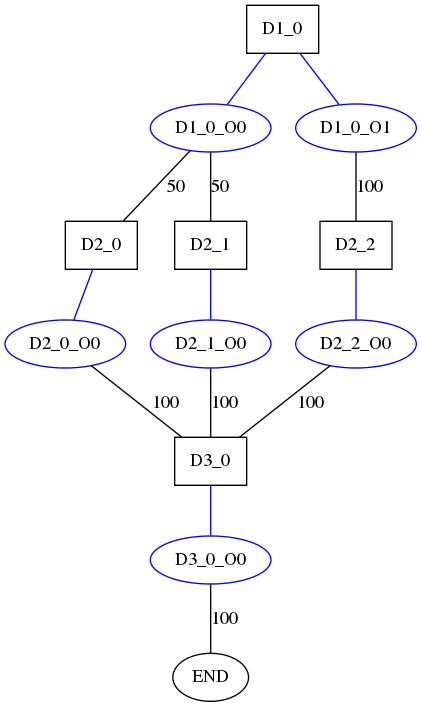
\includegraphics[scale=0.4]{storygraph.png}
 \end{center}
 
 \section{dbtool.py}
 Once a story has been completed and sanity tested, it is necessary to convert its contents into a series of 
 SQL statements for insertion into the Nudge story database. dbtool is used to perform this conversion.
 
 \subsection{Running dbtool}
 dbtool produces a series of SQL statements. As such, it is likely useful to redirect this output to a file that can 
 be sourced later on.
 
 \begin{center}
 dbtool.py mystory.xml $>$mystory.sql
 \end{center}
 
 \subsection{Example output}
 \begin{lstlisting}[breaklines=true]
-- Generated statements for node: D1_0
INSERT INTO storytable VALUES (1,'Example story','D1_0','You are confronted with a serious question: To cheese it or not to cheese it?',0);
INSERT INTO answers VALUES ('Example story','D1_0','A','Cheese it!');
INSERT INTO results VALUES (1,'Example story','D1_0','A',0,50,'D2_0');
INSERT INTO results VALUES (2,'Example story','D1_0','A',50,100,'D2_1');
INSERT INTO answers VALUES ('Example story','D1_0','B','Don\'t cheese it!');
INSERT INTO results VALUES (3,'Example story','D1_0','B',0,100,'D2_2');
-- Generated statements for node: D2_0
INSERT INTO storytable VALUES (2,'Example story','D2_0','You were able to cheese it!',1);
INSERT INTO answers VALUES ('Example story','D2_0','A','Proceed');
INSERT INTO results VALUES (4,'Example story','D2_0','A',0,100,'D3_0');
-- Generated statements for node: D2_1
INSERT INTO storytable VALUES (3,'Example story','D2_1','You were unsuccessful at cheesing it!',2);
INSERT INTO answers VALUES ('Example story','D2_1','A','Proceed');
INSERT INTO results VALUES (5,'Example story','D2_1','A',0,100,'D3_0');
-- Generated statements for node: D2_2
INSERT INTO storytable VALUES (4,'Example story','D2_2','You proceed not to cheese it. This is an additional line to test the parser. Yet another line!',3);
INSERT INTO answers VALUES ('Example story','D2_2','A','Proceed');
INSERT INTO results VALUES (6,'Example story','D2_2','A',0,100,'D3_0');
-- Generated statements for node: D3_0
INSERT INTO storytable VALUES (5,'Example story','D3_0','Regardless of whether you cheesed it, something happened.',4);
INSERT INTO answers VALUES ('Example story','D3_0','A','End');
INSERT INTO results VALUES (7,'Example story','D3_0','A',0,100,'END');
 \end{lstlisting}
 
 \end{document}